

\documentclass{article}        % Your input file must contain these two lines 
\usepackage{bm}
\usepackage{graphicx}
\usepackage{subfigure}
\usepackage{amsmath}
\usepackage{esint}

\title{A note on the fracture flow problem solved by the finite volume method (FVM)}
\author         {Tingchang Yin \\School of Engineering, Westlake University, Hangzhou, China\\yintingchang@foxmail.com}

\date{\today}  
    


\begin{document}               % plus the \end{document} command at the end.
\maketitle
\begin{abstract}
	The steady-state flow is solved by the FVM on unstructured mesh.
\end{abstract}
\section{Governing laws}
The governing equation is
\begin{equation}
k\bm{\Delta} h + F = 0, 
\end{equation}
where $h$ is the hydraulic head, $k$ is the fracture conductivity (here it is assumed to be isotropic), and $F$ is the source term.

\section{Control volume}
Let $\Omega$ denotes the fracture domain, and a mesh consisting of triangles is generated. Here, I use the cell centered FVM, i.e. the barycenter of triangles are the nodes storing the head field. One example is shown in Fig. \ref{controlvolume}. Generally, the node should be the circumcenter of the triangular cell, but if thin triangle exists, the circumcenter may be outside the triangle. The use of barycenter may cause that the connection between two nodes of adjacent cells is not perpendicular to the shared edge, e.g. $E_2, P$ and $v_2,v_3$.

\begin{figure}[htb]
	\centering
	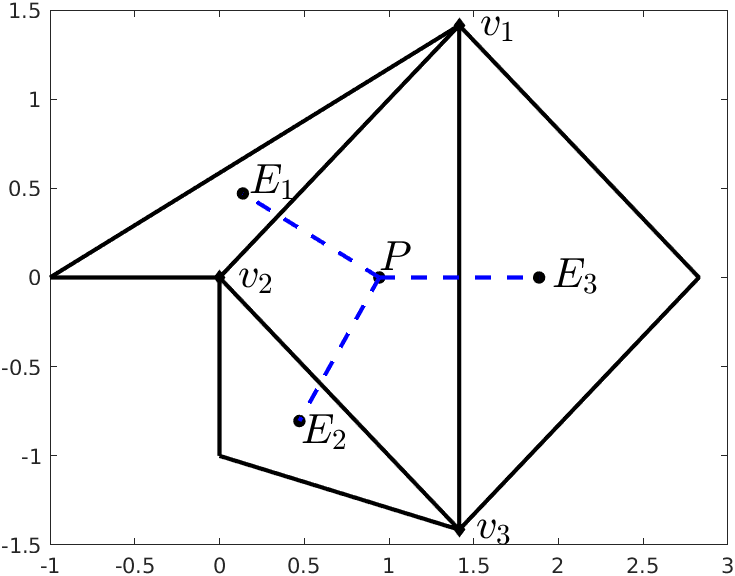
\includegraphics[scale=0.4]{figures/self_center_control_volume.png}
	\caption{The control volume of the barycenter $P$ of a triangle. The volume is surrounding by three triangles.}
	\label{controlvolume}
\end{figure} 

Let us integrate the governing equation over the control volume. The integral is 
\begin{equation}
	k\int_{\Delta V} \bm{\Delta} h \mathrm{d}V + \int_{\Delta V} F \mathrm{d}V = 0,
\end{equation}
where $\Delta V$ is the volume of the cell. By using Green's formula, the integral can be rewritten as
\begin{equation}
k\oint_{\Delta S} \bm{n} \cdot \bm{\nabla} h \mathrm{d}S + \Delta V \cdot \bar{F} = 0,
\end{equation}
where $\Delta S$ is the surfaces of the cell, and $n$ is the inward normal vector of the surfaces. Since a triangle has three edges, we have
\begin{equation}
	\sum_{g = 1}^{3} A_g \cdot \bm{n_g} \cdot \bm{\nabla}h +\Delta V \bar{F} = 0, 
	\label{summation_flux}
\end{equation}
where $A_g$ is the area of the cell edges. This summation hints that the flux through a cell is conserved over $\Delta V$, because $\bm{n_g} \cdot \bm{\nabla}h$ is the scalar flux though each edge.

The summation should be discretized. The Fig. \ref{controlvolume} is taken as example. Let us first consider the flux though edge $v_1, v_2$, which is 
\begin{equation}
 A_{v_1,v_2} \cdot q_{\perp v_1,v_2}, \notag
\end{equation}
and $q_{\perp v_1,v_2}$ is the flux rate. Let$\theta_1$ denotes the angle between the inward normal vector of edge $v_1,v_2$ and the line segment $E_1, P$, and subsequently we have
\begin{equation}
	q_{\perp v_1,v_2} = q_{E_1, P} \cdot \cos{\theta_1},\notag
\end{equation}
and $q_{E_1, P}$ is the scalar flux rate along line segment $q_{E_1, P}$. The $q_{E_1, P}$ can be approximated now as:
\begin{equation}
	k\cdot \frac{h_{E_1} - h_{P}}{l_{E_1, P}}, \notag
\end{equation}
and $l_{E_1, P}$ is the length of the line segment $E_1, P$.

In a similar way, the Eq. (\ref{summation_flux}) can be rewritten as
\begin{equation}
	k\sum_{g = 1}^{3}A_g \cdot \frac{h_{E_g}-h_P}{l_{E_g,P}}\cdot \cos{\theta_g} + \bar{F}\cdot \Delta V = 0.
\end{equation}
Let us sort this equation: for node $P$ (or $h_P$), the coefficient is given by
\begin{equation}
\alpha_P = k\sum_{g = 1}^{3} A_g\cdot \frac{-1}{l_{E_g, P}}\cdot \cos{\theta_g}, \notag
\end{equation}
and for each $E_g$, the coefficient is
\begin{equation}
	\alpha_g = k \cdot A_g \cdot \frac{1}{l_{E_g, P}} \cdot \cos{\theta_g}, g \in[1,3]. \notag
\end{equation} 
The source term is generally linearized:
\begin{equation}
 \bar{F} \cdot \Delta V = F_u + F_P\cdot h_P. \notag
\end{equation}
Therefore, the simplified form of the Eq. (\ref{summation_flux}) is
\begin{equation}
	(-\alpha_P - F_P)\cdot h_P = \sum \alpha_g \cdot h_{E_g} + F_u,
	\label{simplified_coe}
\end{equation}
where $g \in [1,3]$. If $F$ is a constant, then $F_u = F$ and $F_P = 0$.

\section{Control volume of boundary cells}
This note involves the consideration of two kinds of boundary conditions. The first one is the Dirichlet condition:
\begin{equation}
h = h_D \text{ on } \Gamma_D,	
\end{equation}
where $\Gamma$ is the considered boundary. The another one is the Neumann condition:
\begin{equation}
	\bm{\nabla} h \cdot \bm{n} = 0 \text{ on } \Gamma_N.
\end{equation}

\begin{figure}[htb]
	\centering
	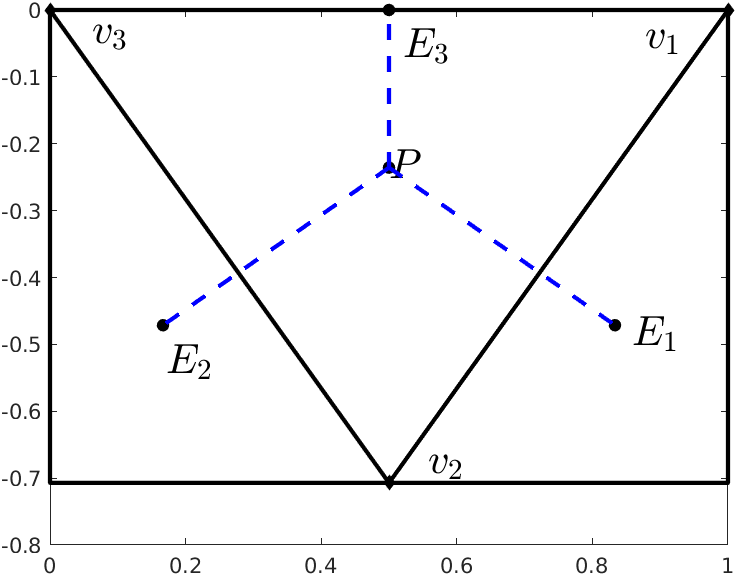
\includegraphics[scale=0.4]{figures/1st_bc.png}
	\caption{A cell containing a boundary edge $v_3, v_1$.}
	\label{1st_bc}
\end{figure}

Let us consider the Dirichlet condition first. One example is shown is Fig. \ref{1st_bc}. In this circumstance, the flux through edge $v_3,v_1$ is
\begin{equation}
	q_{E_3, P} = k \cdot \frac{h_D - h_P}{l_{E_3, P}}, \notag
\end{equation}
but the $\alpha_3$ is set to zero and $g$ is in $[1,2]$. The $F_u$ here is given by
\begin{equation}
F_u = A_3 \cdot k\cdot \frac{h_D}{l_{E_3, P}}, \notag	
\end{equation}
and $F_P$ is
\begin{equation}
	F_P = A_3\cdot k \cdot\frac{-1}{l_{E_3, P}}. \notag
\end{equation}
In this way, the Eq. (\ref{simplified_coe}) can be rewritten as
\begin{equation}
	(-\alpha_P - F_P)\cdot h_P = \sum \alpha_g \cdot h_{E_g} + F_u, g \in [1,2],
\end{equation}
and the original form is still preserved.

Then, we should turn to the Neumann condition. If the $q_{\perp v3,v1}$ is set to zero, then we have
\begin{equation}
k\sum_{g = 1}^{2}A_g \cdot \frac{h_{E_g}-h_P}{l_{E_g,P}}\cdot \cos{\theta_g} + k \cdot A_3 \cdot q_{\perp v3,v1}  + \bar{F}\cdot \Delta V = 0. \notag
\end{equation}
In this condition, we can deem $F_u = k \cdot A_3 \cdot q_{\perp v3,v1} = 0$ and then have
\begin{equation}
(-\alpha_P - F_P)\cdot h_P = \sum \alpha_g \cdot h_{E_g} + F_u, g \in [1,2],
\end{equation}
where $F_P = 0$, and $\alpha_P$ is
\begin{equation}
	\alpha_P = k\sum_{g = 1}^{2} A_g\cdot \frac{-1}{l_{E_g, P}}\cdot \cos{\theta_g}. \notag	
\end{equation}
Still, the simplified form is preserved.


 

\end{document}

